\documentclass[12pt]{article}

\usepackage[spanish]{babel}
\usepackage[utf8]{inputenc}
\usepackage{graphicx}
\usepackage{geometry}
\usepackage{xcolor}
\usepackage{fancyhdr}
\usepackage{lastpage}
\usepackage{pdfpages}
\usepackage{listings}
\usepackage{schemata}

\geometry{top=25mm,left=15mm,right=15mm,a4paper}

\pagestyle{fancy}
\fancyhf{}
\lhead{Redes de Computadoras}
\cfoot{Página \thepage\ de \pageref{LastPage}}

\graphicspath{./}

\begin{document}
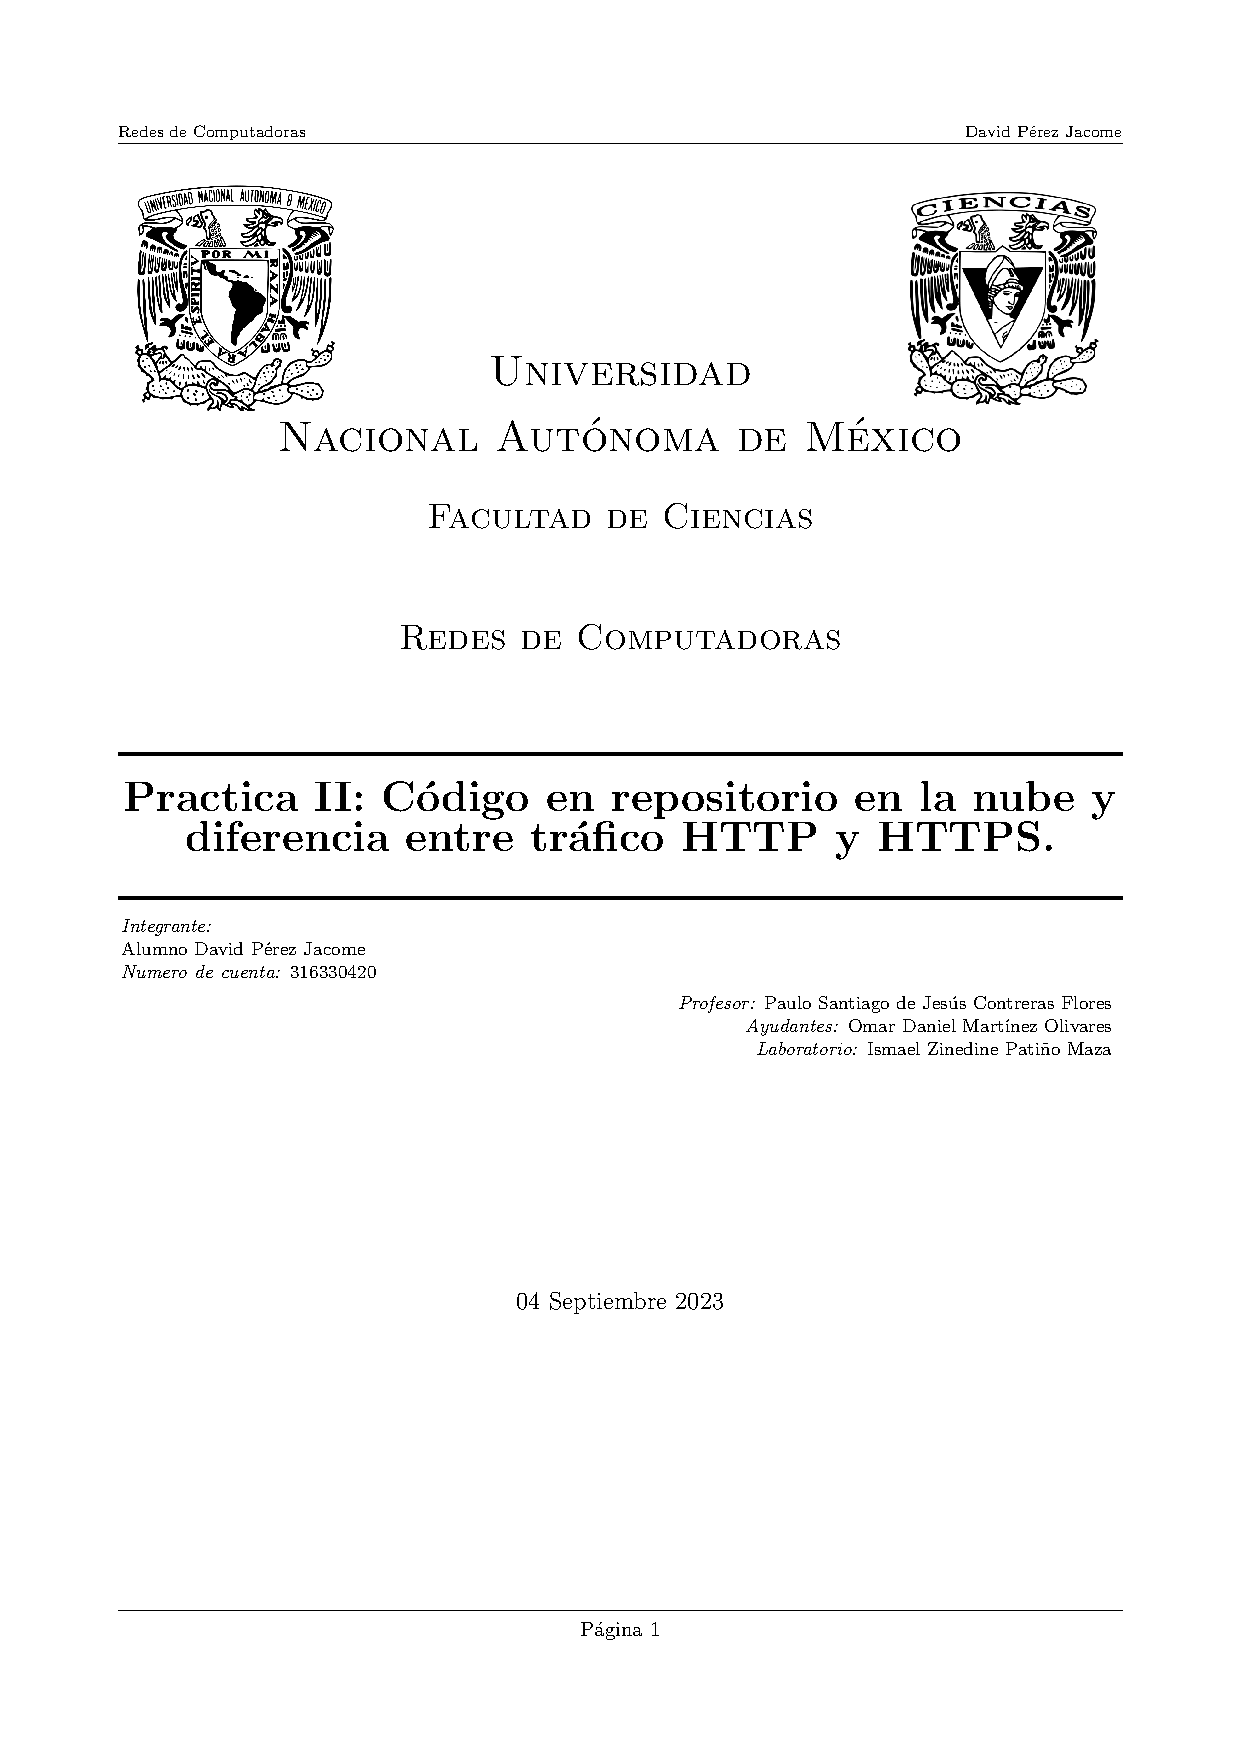
\includepdf{Portada.pdf}
{\color{red} \section*{\textbf{Practica II: Código en repositorio en la nube y diferencia entre tráfico HTTP y HTTPS.}}}
\vspace{1em}

{\color{blue} \subsection*{\textbf{Objetivo.}}}
\vspace{1em}
El alumno centralizará el código fuente de un proyecto web en la nube con Git (GitLab), adicionalmente visualizará la diferencia entre tráfico HTTP y HTTPS.
\vspace{2em}


{\color{blue} \subsection*{\textbf{Desarrollo.}}}
\vspace{1em}
\begin{enumerate}
    \item Crea un fork del repositorio https://github.com/ZizuPM/Practica_2_GPCCrea un fork del repositorio $https://github.com/ZizuPM/Practica_2_GPC$, en tu propia cuenta de Github., en tu propia cuenta de Github.\\
    \textbf{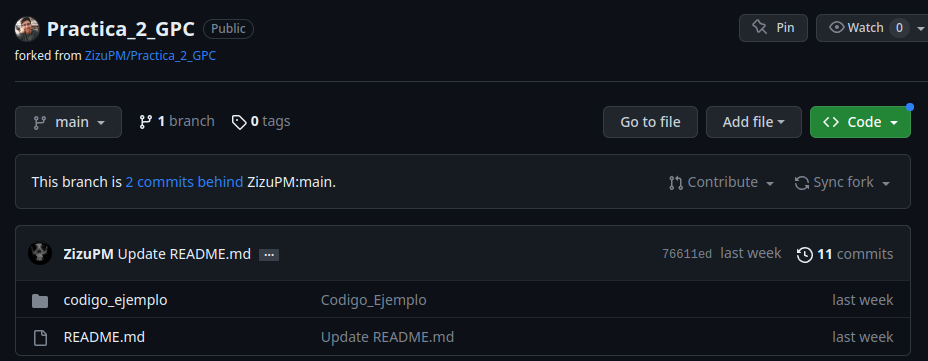
\includegraphics[scale = 0.40]{images/fock en git.png}}\\ Aqui tenemos el fork en el repositorio de la practica.
    \item Ingresa desde una terminal al servidor que instalaste en la Práctica 2, en GCP.\\
    \textbf{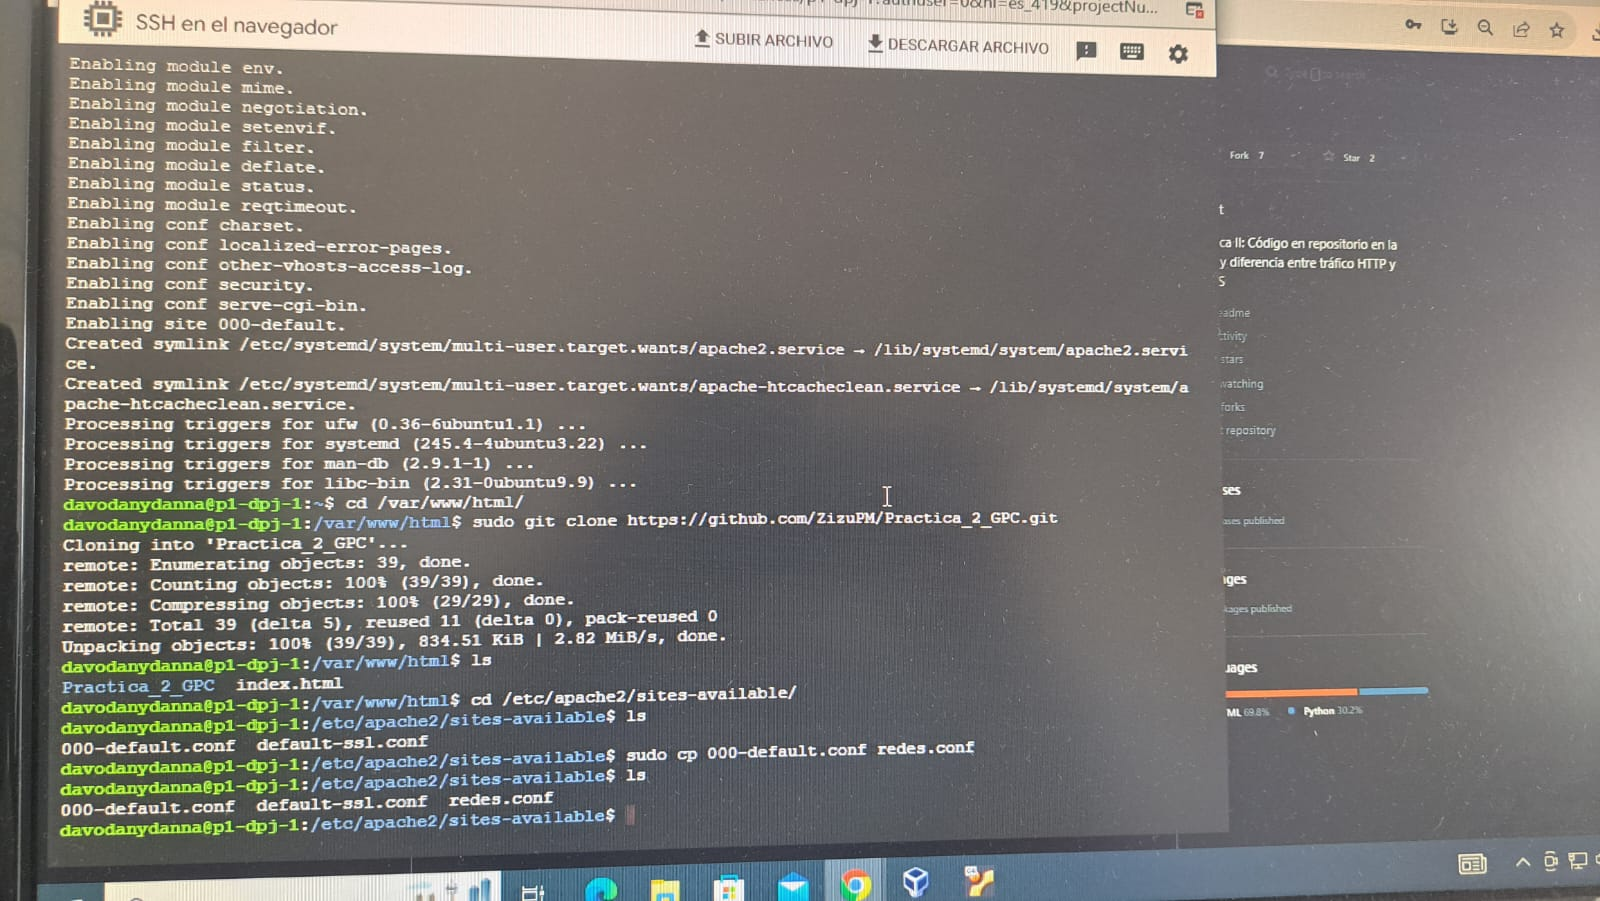
\includegraphics[scale = 0.35]{images/pasooooo.jpeg}}\\ Aqui tenemos la captura de pantalla de nuestra terminal en nuestra maquina virtual ubuntu donde en los siguientes pasos clonaremos el repositorio.\\
    \item Cambia al directorio $/var/www/html$.\\
    \textbf{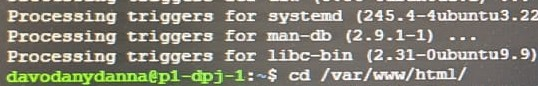
\includegraphics[scale = 0.50]{images/p3.jpeg}}\\ En este paso cambiamos al direcctorio mencionado anteriormente.
    \item Clona tu repositorio creado en el paso 1, con el comando $sudo git clone <https://mi_repositorio>$\\
    \textbf{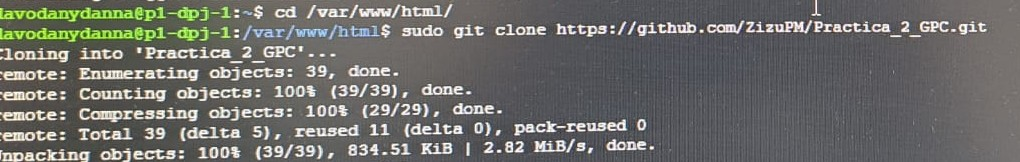
\includegraphics[scale = 0.50]{images/p2.jpeg}}\\ Ahora clonamos el repositorio anteriormente mencionado en nuestra maquina virtual.\\
    \item Cambia al directorio $/etc/apache2/sites-available/$.\\
    \textbf{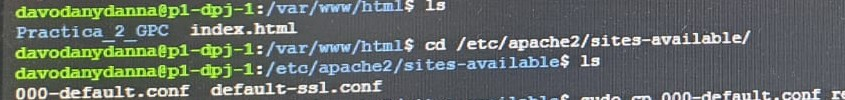
\includegraphics[scale = 0.50]{images/p5.jpeg}}\\ Nos cambiamos a ese directorio y enlistamos los archivos que tenemos en esa ruta.\\
    \item Copia el archivo $000-default.conf$ al archivo $redes.conf$, utiliza la opción $-a$ en el comando $cp$, para que se preserven los atributos del archivo, tales como el dueño, el grupo y los permisos.\\
    \textbf{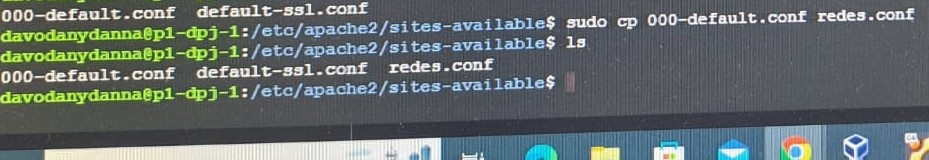
\includegraphics[scale = 0.50]{images/p6.jpeg}}\\ creamos el archivo de nombre \textbf{redes.conf} que en realidad es solo una copia.\\
    \item Con un editor de texto, abre el archivo $redes.conf$ copiado en el paso anterior.\\
    \textbf{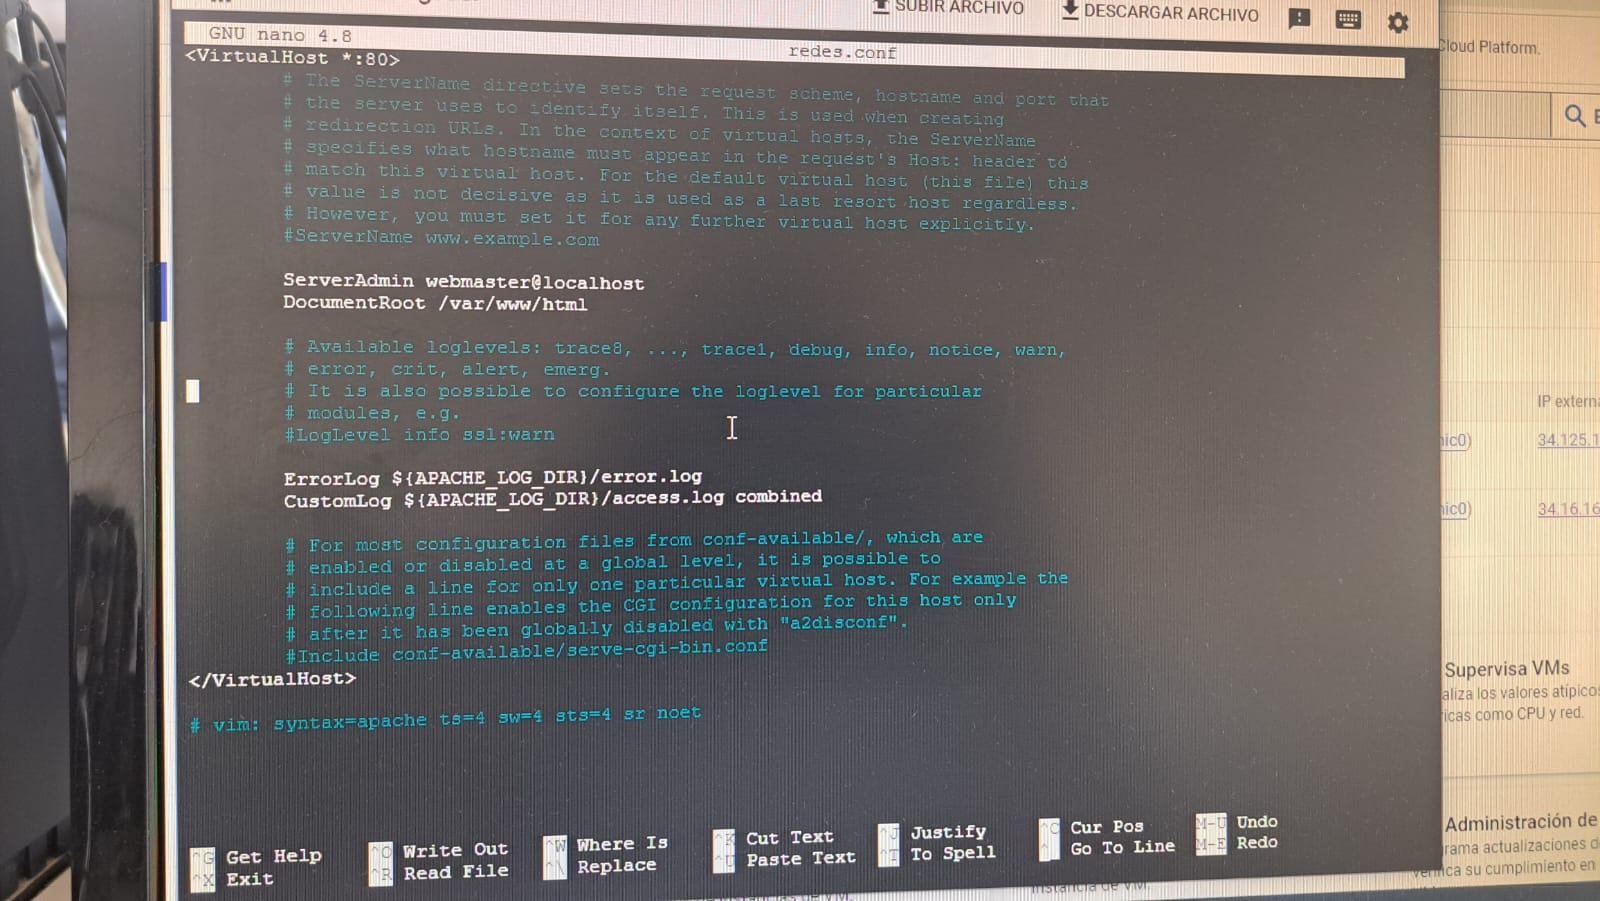
\includegraphics[scale = 0.35]{images/p7.jpeg}}\\ Para editar el texto yo utilice nano como mi editor por sonsola.\\
    \item Cambia el valor de la directiva $DocumentRoot$, en lugar de que esté establecido con la ruta $/var/www/html$, coloca la ruta en donde se encuentra el código HTML y otros elementos web de la carpeta $codigo_ejemplo/$ de la práctica 2 del repositorio clonado en el punto 4.\\
    \textbf{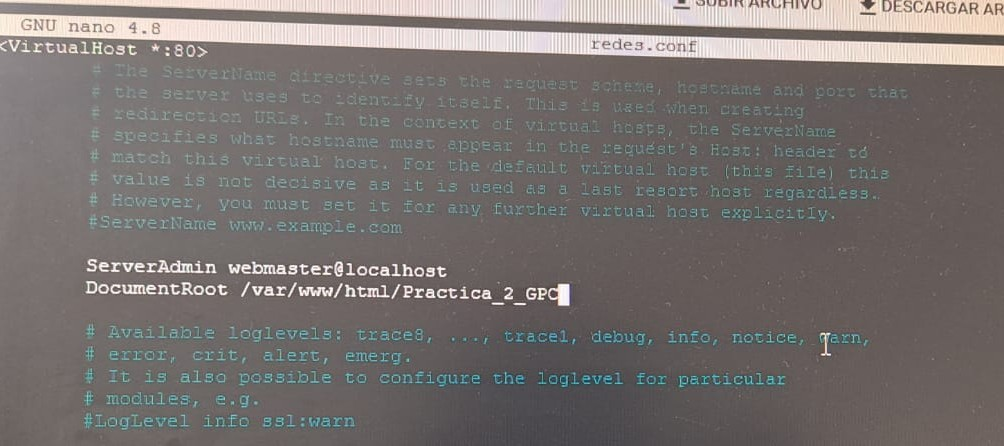
\includegraphics[scale = 0.50]{images/p8.jpeg}}\\ Aqui editamos el documento con la ruta $Practica_2_GPC$.\\
    \item Guardamos los cambios en el archivo.\\
    \item Cambiamos al directorio $/var/www/html/Practica_2_GPC/$.\\
    \item Cambiamos tanto el usuario como el grupo del directorio y de sus elementos, por mi usuario, Todos los pasos anteriores se puede ver en la siguiente captura de pantalla.\\
    \textbf{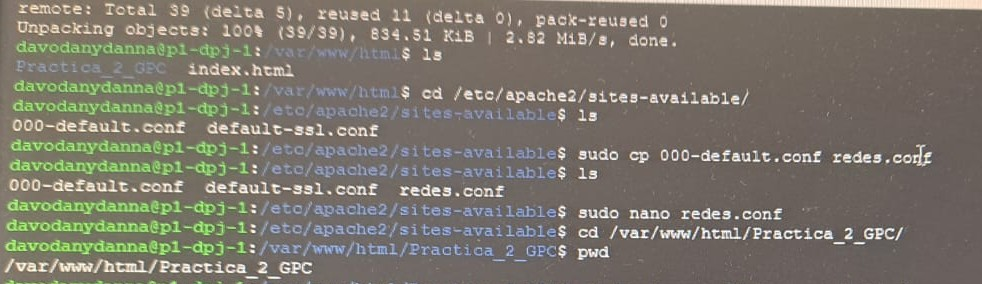
\includegraphics[scale = 0.50]{images/p11.jpeg}}\\
    \item En la terminal ejecutamos el comando $sudo a2dissite 000-default.conf$ para deshabilitar el sitio actual. Y ejecutamos el comando $sudo a2ensite redes.conf$, para habilitar el nuevo sitio web. Para verificar si la configuración creada es correcta ejecutamos $apachectl -t$ lo cual nos dira si el archivo es correcto y para que se apliquen los cambios reiniciamos el servidor Apache.\\
    \textbf{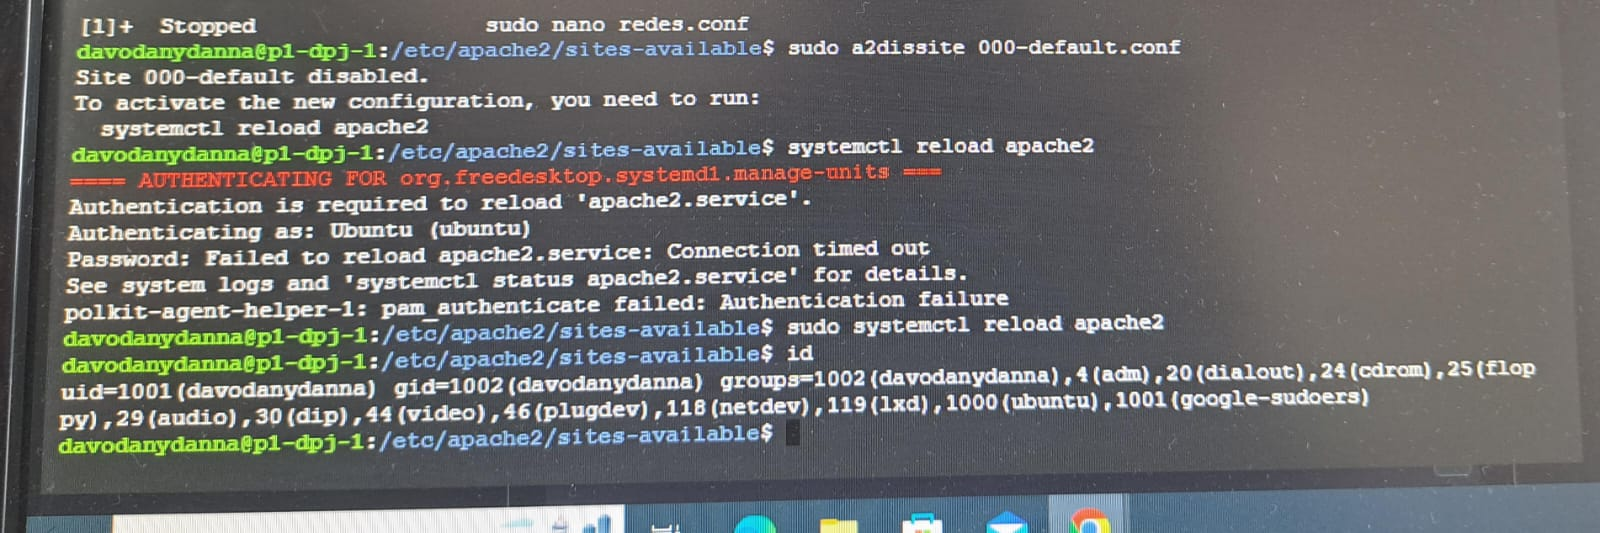
\includegraphics[scale = 0.50]{images/p12.jpeg}}\\
    \textbf{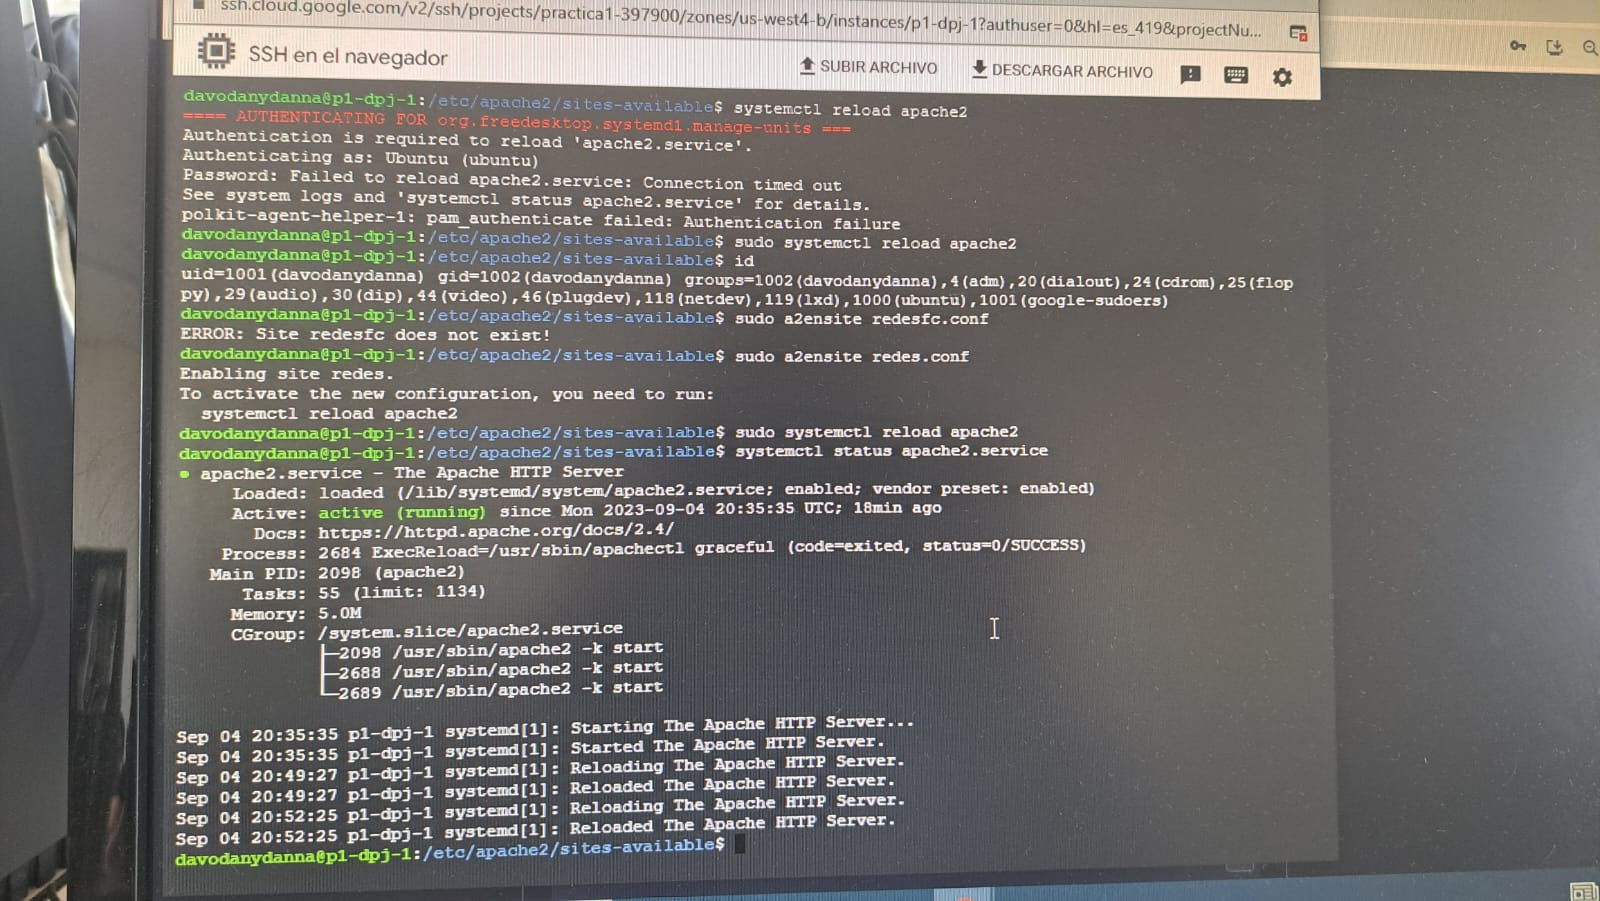
\includegraphics[scale = 0.50]{images/p12-2.jpeg.jpeg}}\\ Aqui una imagen del servicio funcionando.\\
    \item Ingresamos desde un navegador web usando la dirección IP pública proporcionada por GCP, al servidor web donde vemos un formulario, seguido de ello entramos a  $http://mi_IP/images$.\\
    \textbf{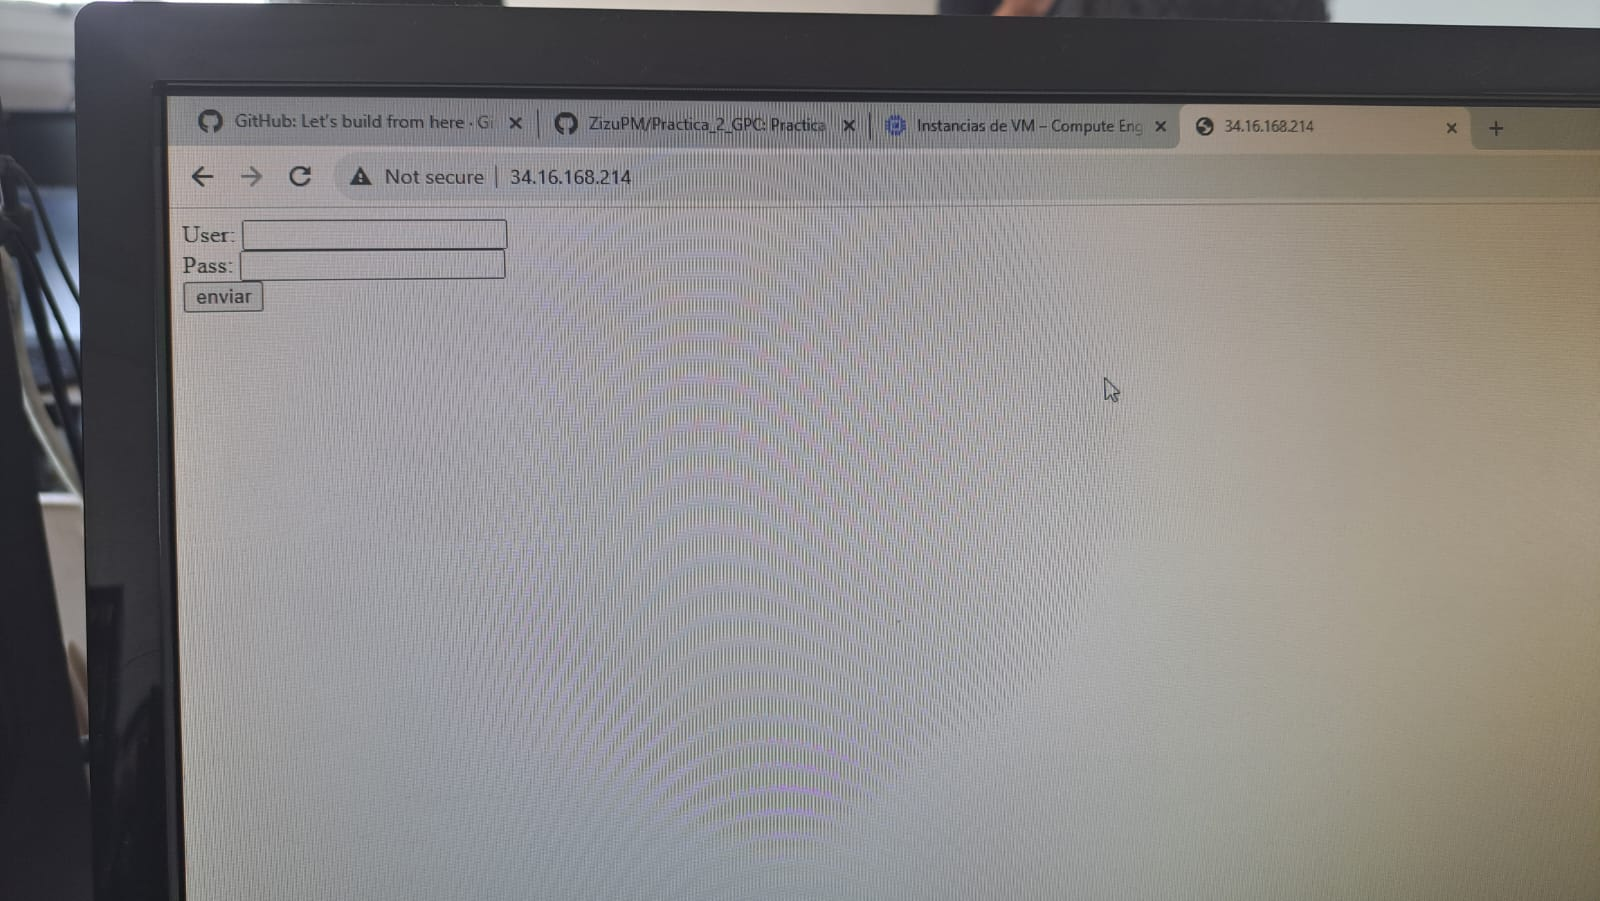
\includegraphics[scale = 0.30]{images/p13.jpeg}}\\ Aqui el formulario\\
    \textbf{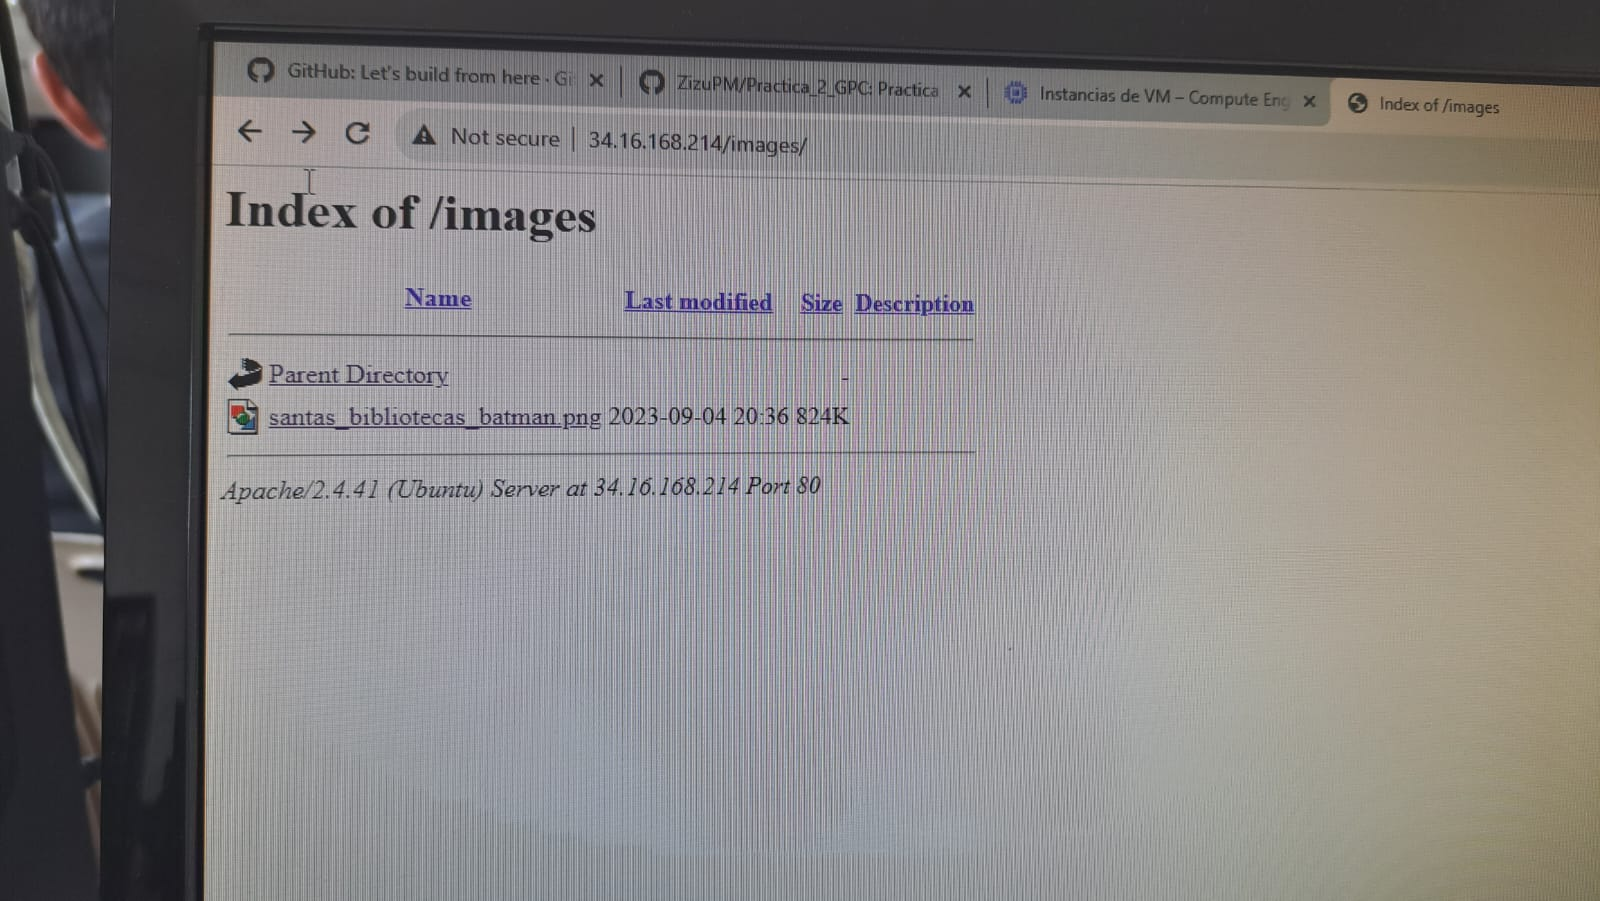
\includegraphics[scale = 0.30]{images/p13-2.jpeg}}\\ la parte de images.\\
    \textbf{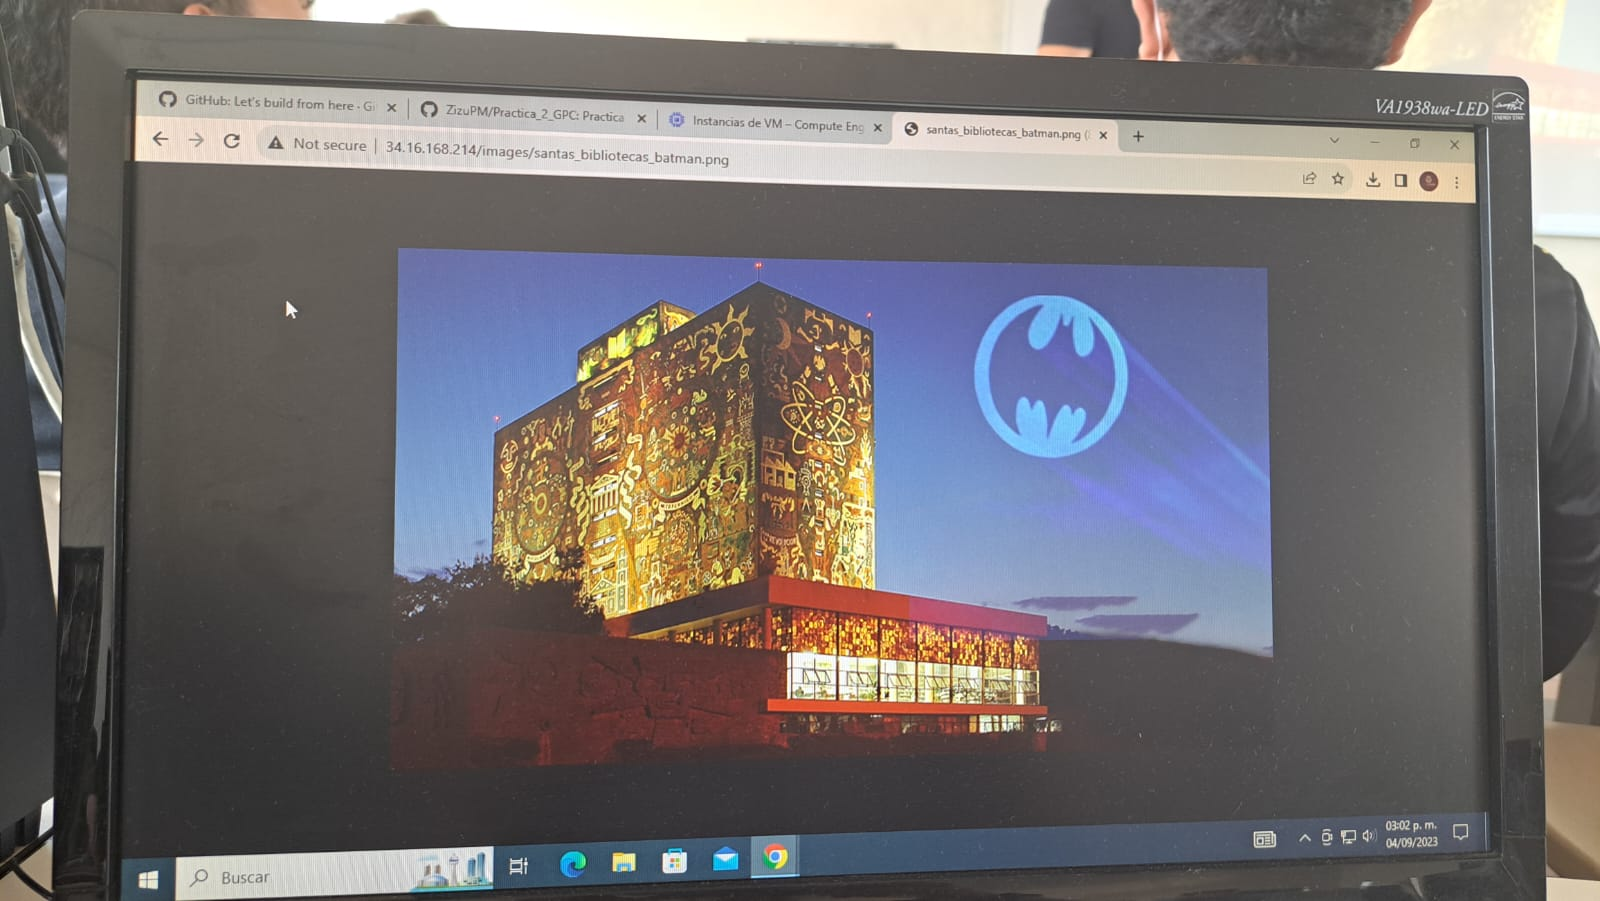
\includegraphics[scale = 0.30]{images/p13-3.jpeg}}\\ La imagen de Batman.\\
    \item En el mismo archivo $redes.conf$, agregamos entre las directivas $<VirtualHost></VirtualHost>$. Verificamos que la ruta del directorio sea el correcto para evitar que el servidor liste el contenido de los directorios de la ruta configurada en DocumentRoot, es una configuración de seguridad.\\
    \textbf{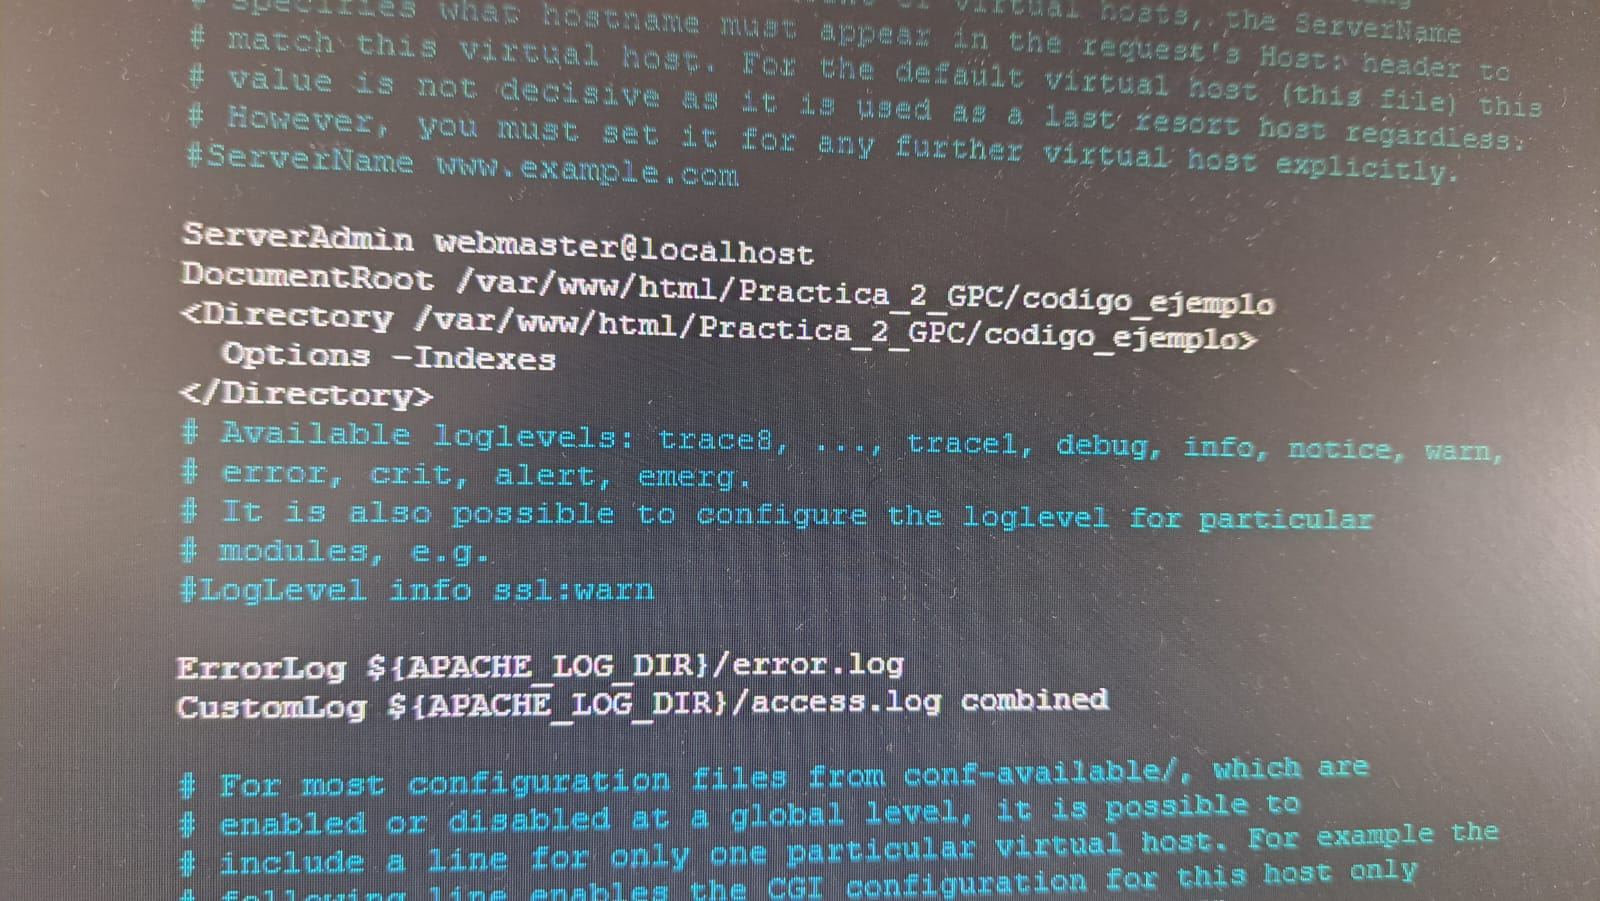
\includegraphics[scale = 0.50]{images/p14.jpeg}}\\ Nos aseguramos que esten ambas en GPC, ya que por ello no nos jalaba al inicio.\\
    \item Para que se apliquen los cambios ejecutamos el comando $sudo systemctl restart apache2.service.$\\
    \item Ingresamos de nuevo a la ruta $http://mi_IP/images$, y observamos que ahora no podemos ingresar a la imagen de batman, ya nos queda como restringido.\\
    \textbf{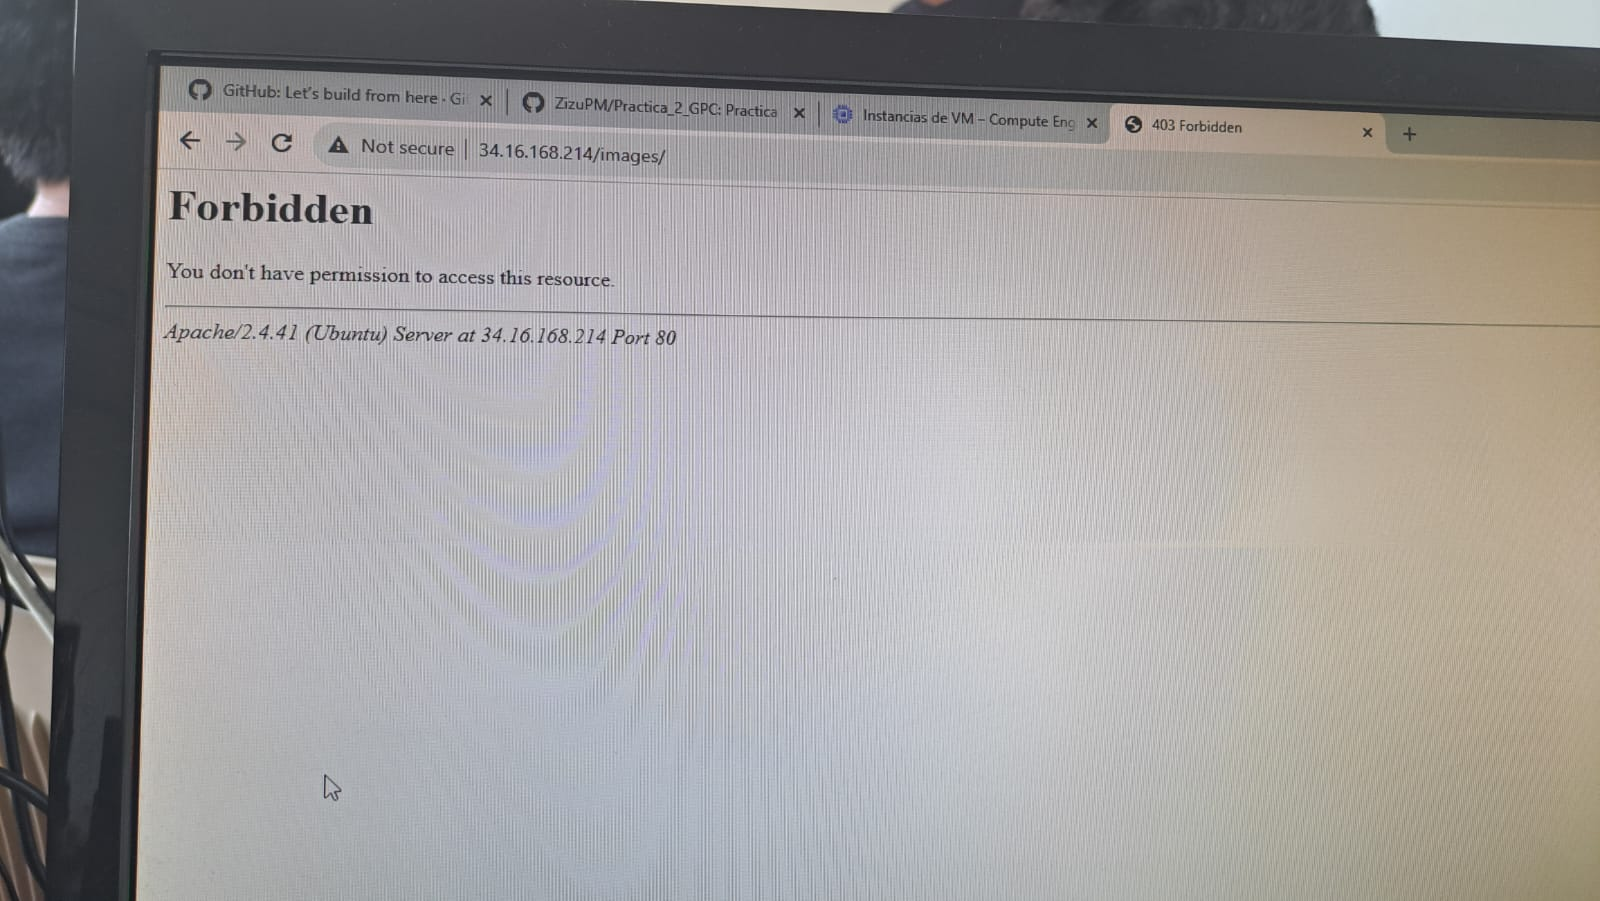
\includegraphics[scale = 0.30]{images/p16.jpeg}}\\
    \item Ejecutamos ahora  el comando $sudo a2enmod cgid$, para habilitar el módulo de Apache de ejecución de CGI.\\
    \textbf{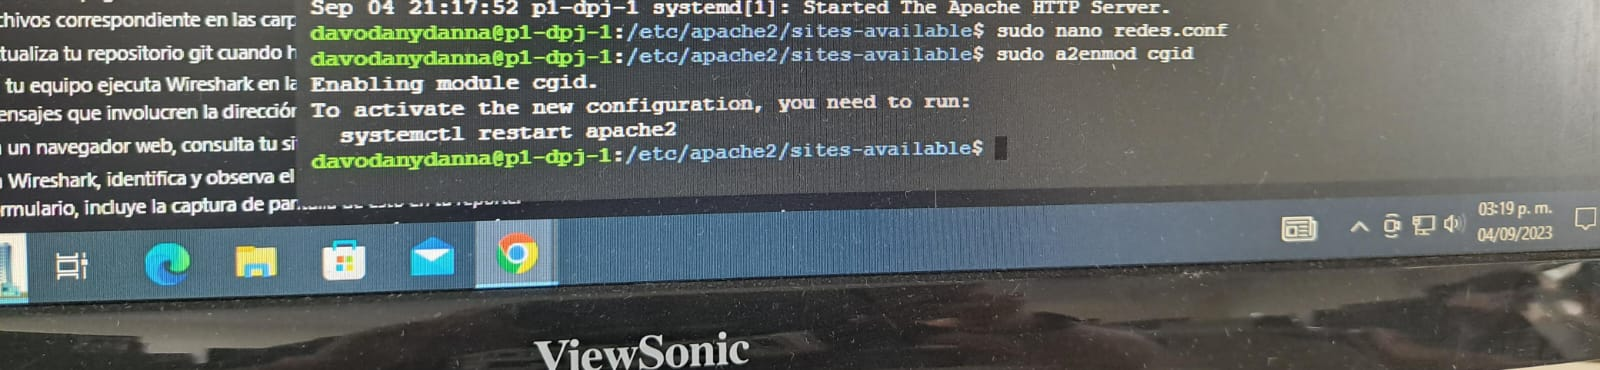
\includegraphics[scale = 0.55]{images/p17.jpeg}}\\
    \item Ahora en redes.conf, agregamos el codigo de la pagina para configurar la ejecución de scripts de Python en el directorio en donde está el repositorio de git.\\
    \textbf{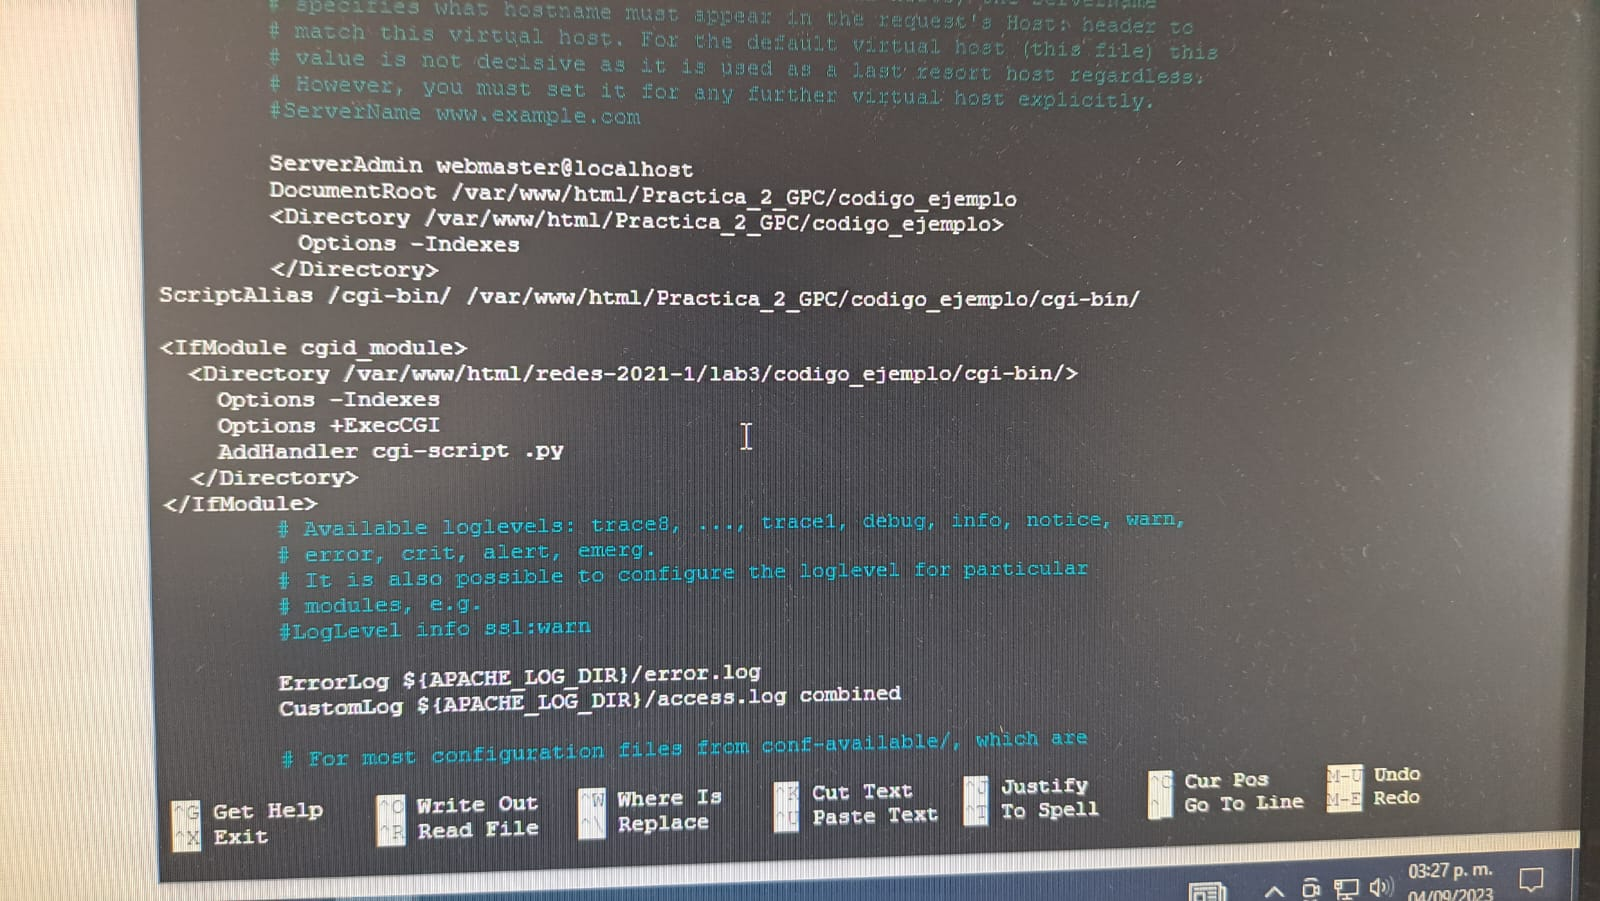
\includegraphics[scale = 0.30]{images/p18.jpeg}}\\ igual debemos de tener cuidado que sea igual al host.\\
    \textbf{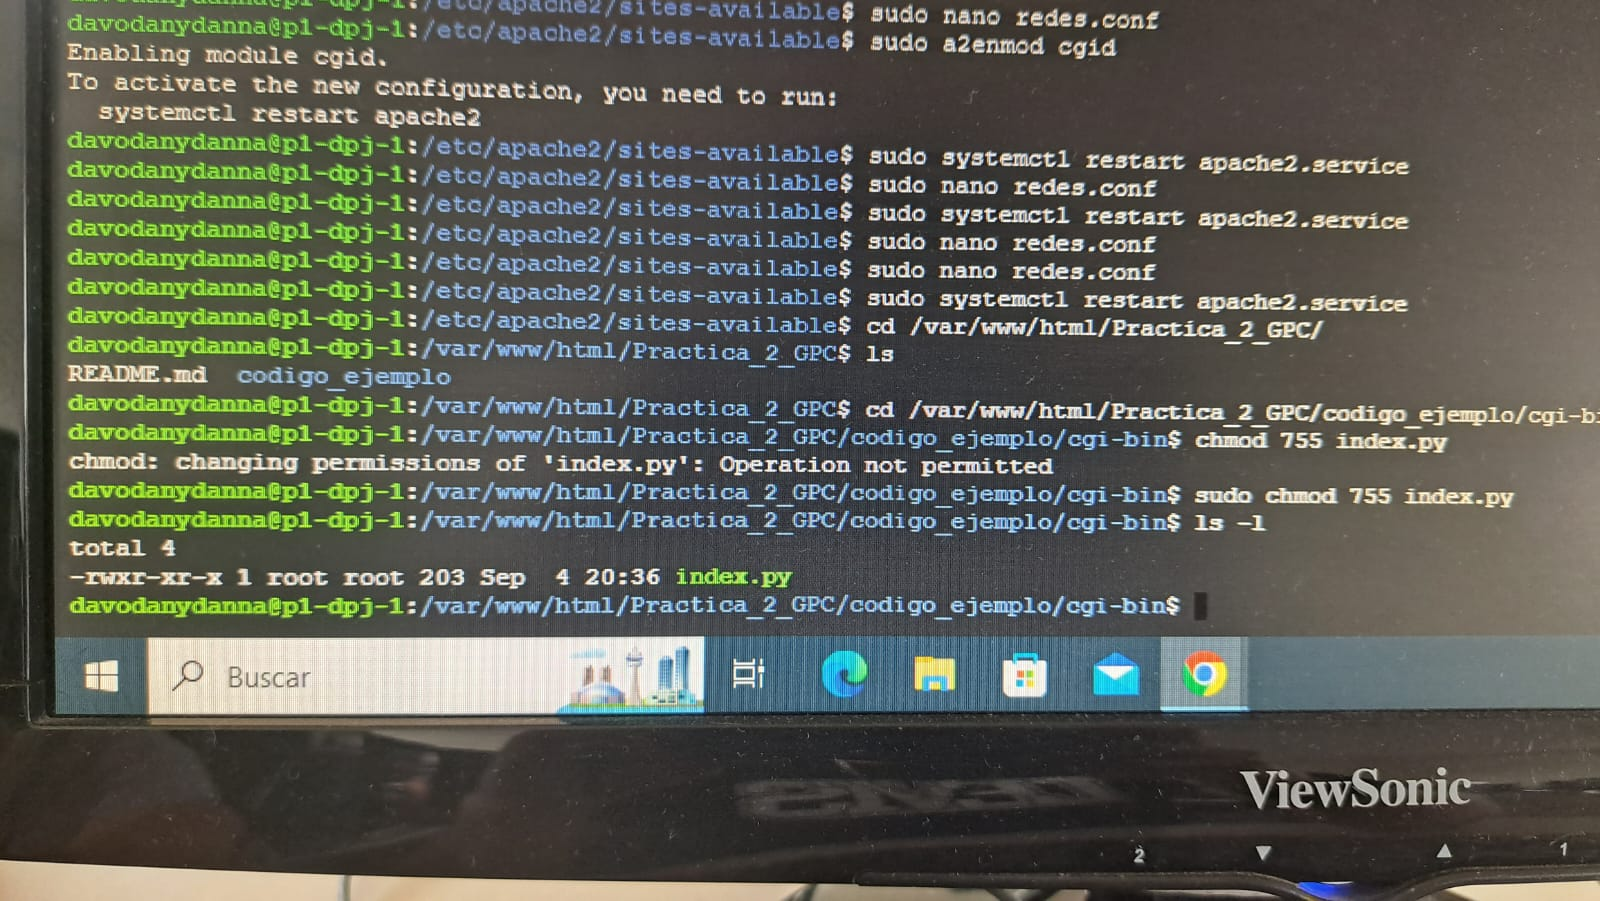
\includegraphics[scale = 0.30]{images/p19-2.jpeg}}\\
    \item Ingresamos al formulario desde un navegador web, y verificamos que se esté ejecutando correctamente el script de Python.\\
    \textbf{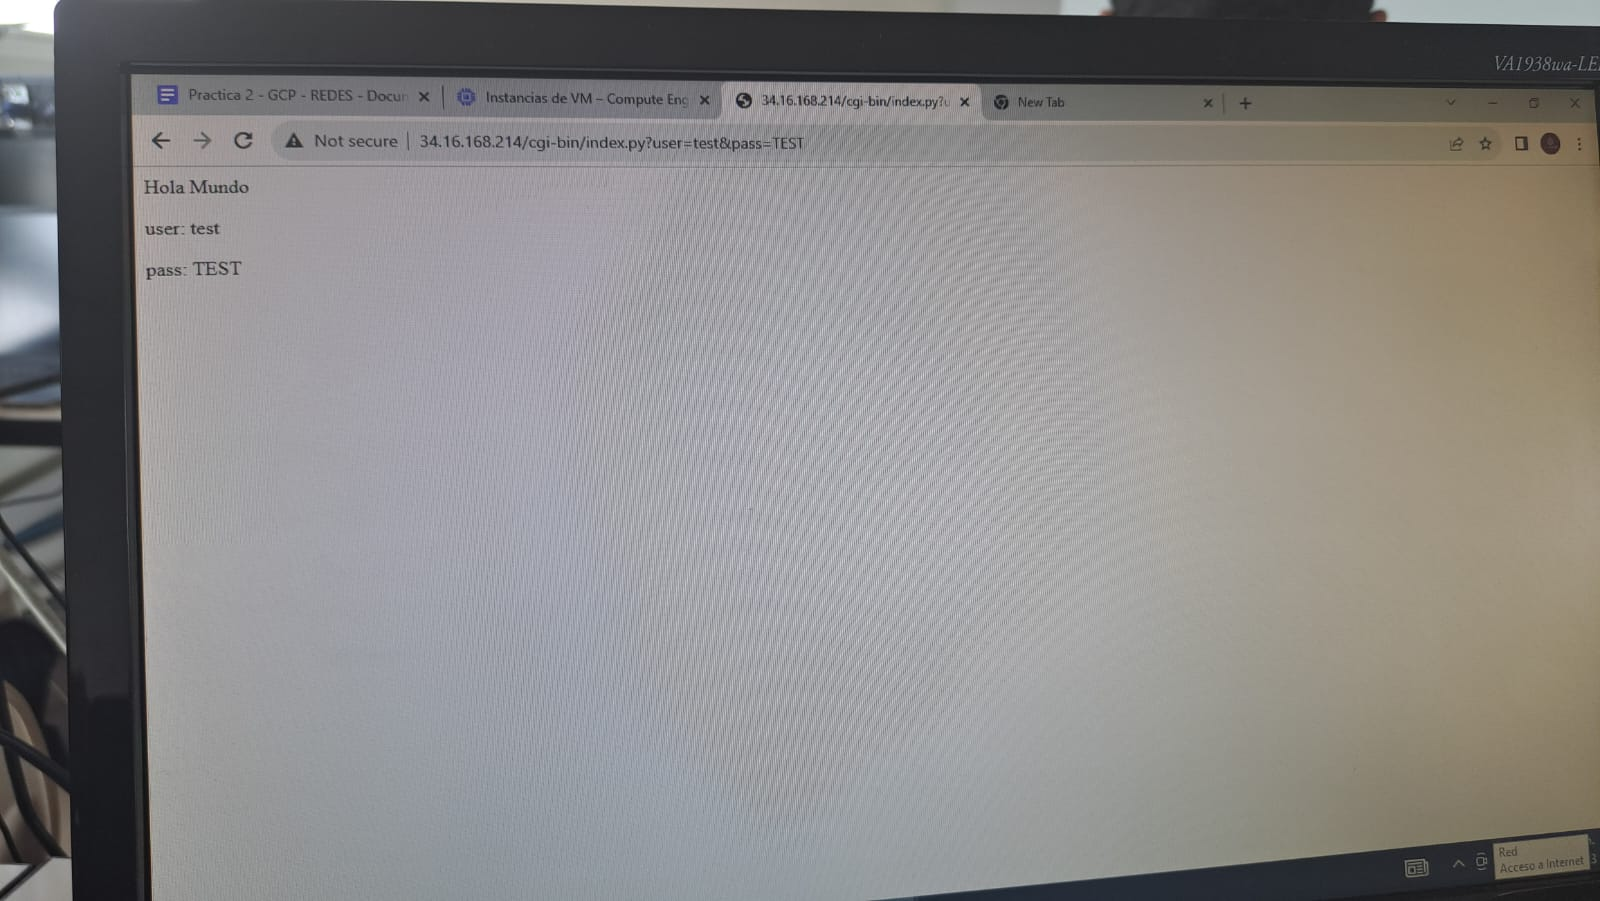
\includegraphics[scale = 0.30]{images/p19.jpeg}}\\
    \item Ahora con la herramienta Wireshark,  capturamos el tráfico de la navegación de acceso al formulario. Para realizar esto seleccionamos la tarjeta de red por la cual capturaremos el tráfico de red, después tendremos que aplicar un filtro el cual capture únicamente el tráfico, posteriormente navegaremos al sitio web donde llenaremos el formulario y lo accionaremos, finalmente analizaremos el tráfico de navegación.\\
    \textbf{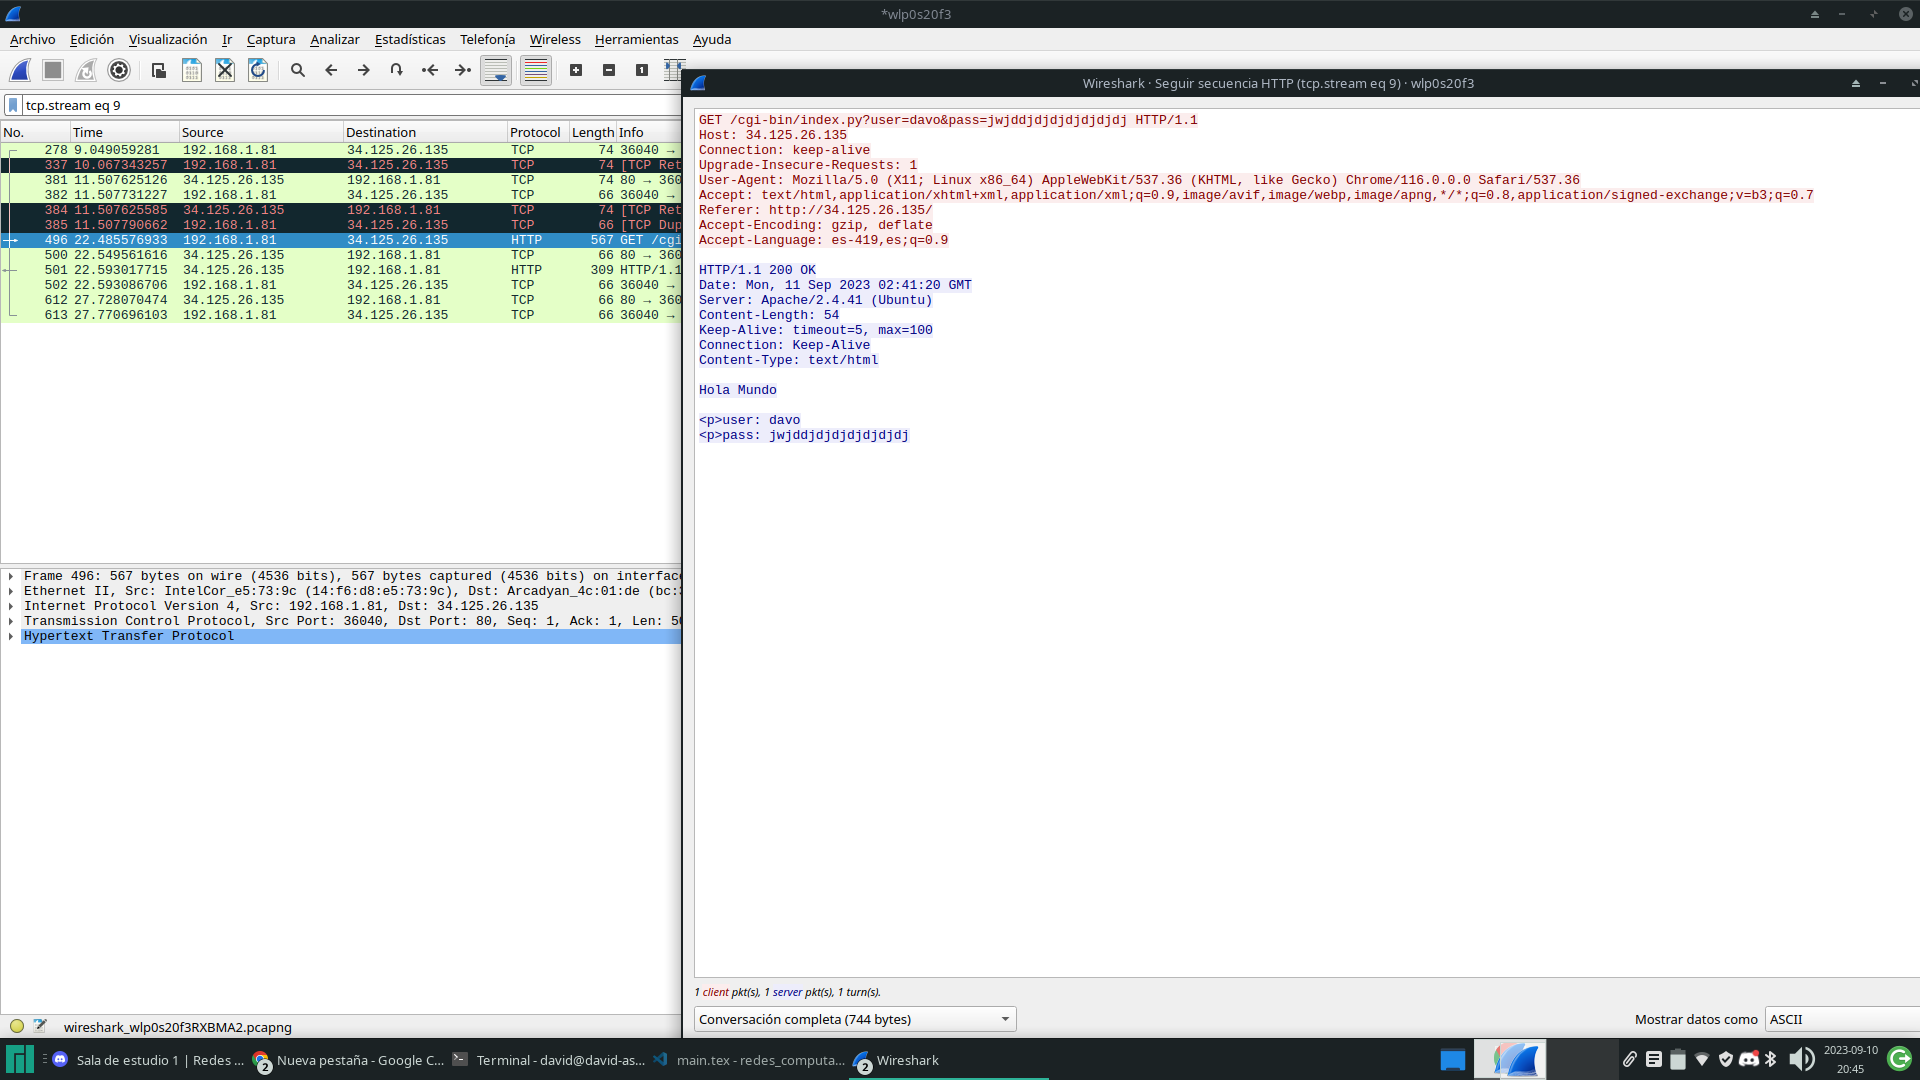
\includegraphics[scale = 0.30]{images/captura de paquetes.png}}\\ Aqui podemos ver que se ve el usuario y la contraseña al capturar los paquetes.\\
\end{enumerate}\\


{\color{blue} \subsection*{\textbf{Evaluación.}}}
\vspace{1em}
\begin{enumerate}
    \item Menciona con tus propias palabras las ventajas que tiene centralizar el código fuente con git sin trabajar directamente en el servidor.\\
    \textbf{Algunas de las ventajas que tenemos es que podemos hacer el control de versiones y podemos hacer modificaciones a nuestro trabajo y despues ya subirlo, otra es que podemos trabajar en equipo con otros compañeros en proyectos grandes, además es más seguro.}\\
    
    \item ¿Para qué se usa la directiva Options -Indexes?\\
    \textbf{Se usa para deshabilitar la funcionalidad de listado de directorios, o sea mejorar la seguridad y la privacidad de un sitio web al evitar que los usuarios puedan ver la lista completa de archivos}\\
    
    \item Liga del repositorio GitLab del repositorio con tus cambios\\
    \textbf{https://github.com/davo1956/Practica_2_GPC}

    \item Captura de pantalla del tráfico http (no seguro) con wireshark, marcando en dónde se envía la información en claro, tanto para el método GET como para el método POST.¿Cuál es la diferencia que se aprecia en Wiresharl entre los mensajes que en donde se usó el método GET y los mensajes en donde se usa el método POST?, ¿cuál es la diferencia que se nota en el navegador web cuando se usa cada uno de estos métodos?\\
    \textbf{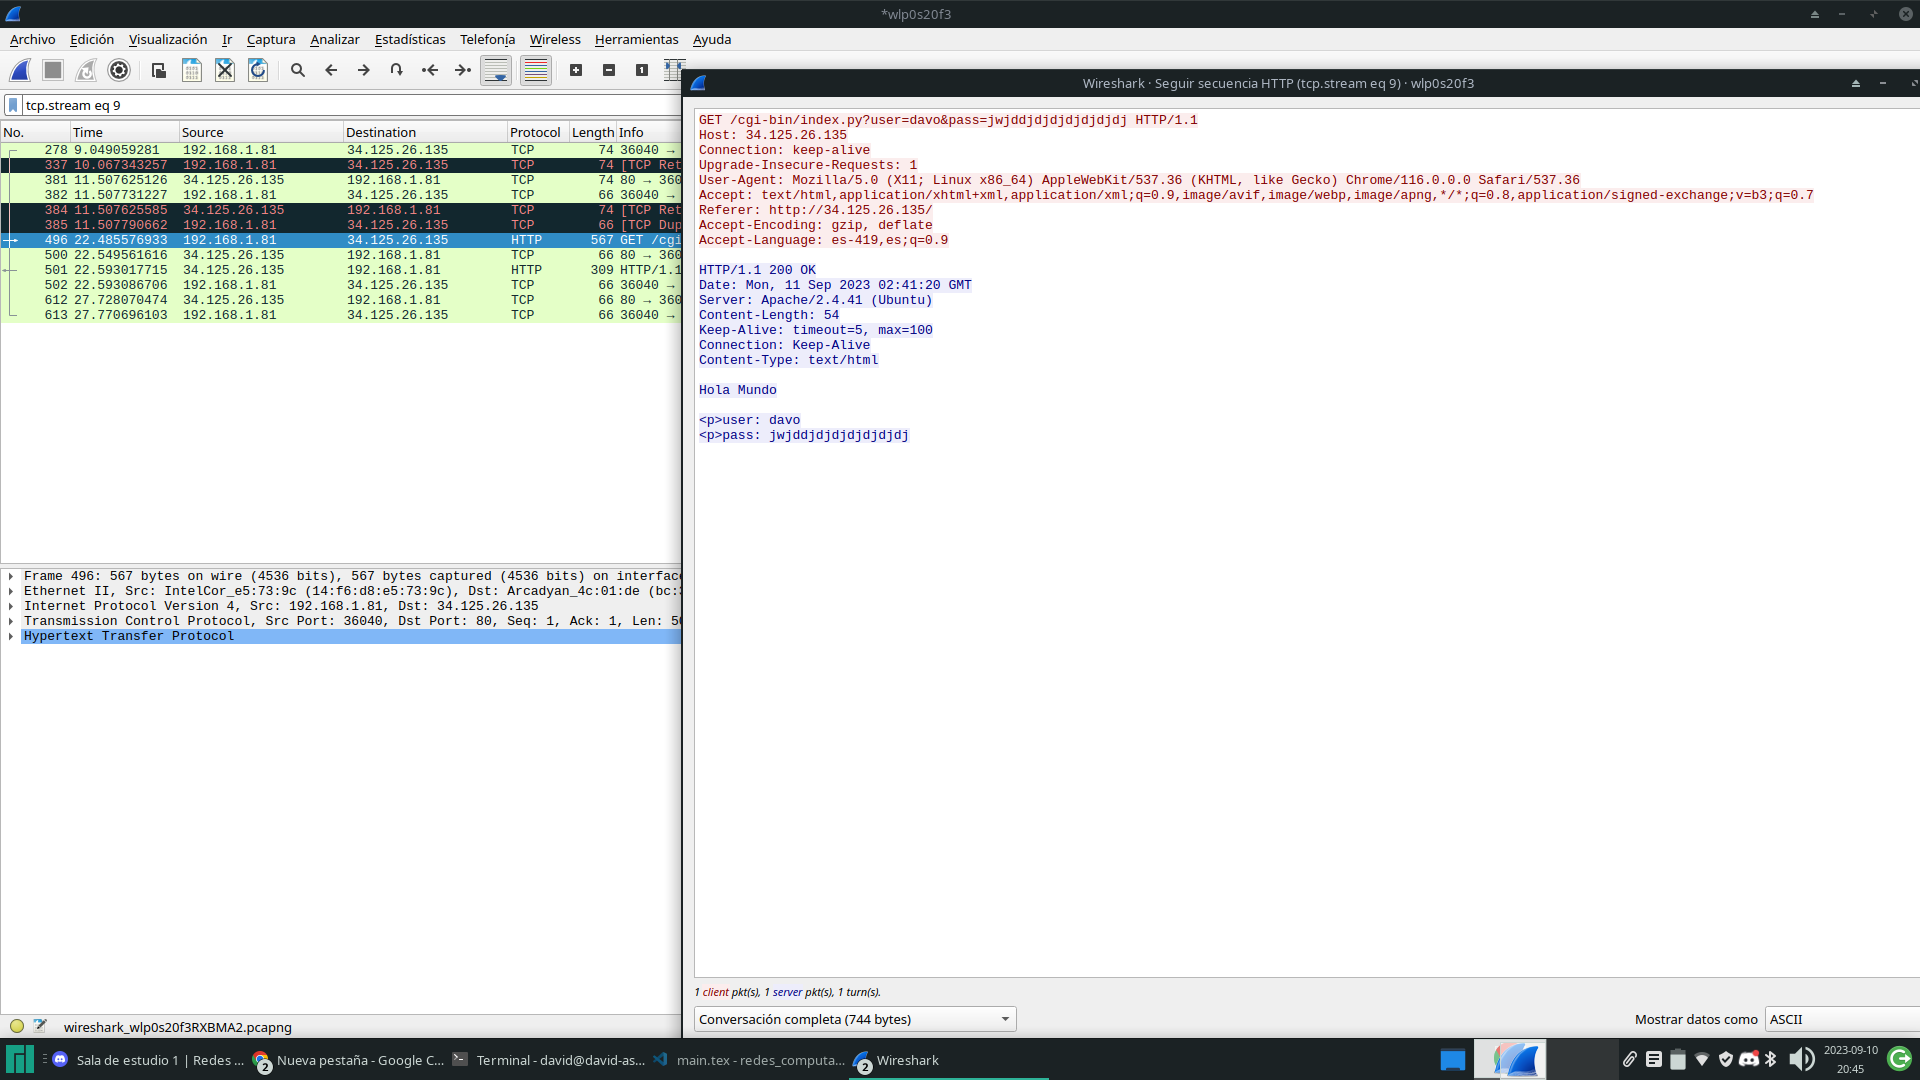
\includegraphics[scale = 0.25]{images/captura de paquetes.png}}\\ l analizar el tráfico de red en Wireshark, puedes diferenciar fácilmente las solicitudes GET de las solicitudes POST observando la ubicación de los datos, la visibilidad de los mismos, el tamaño de los paquetes y, en caso de solicitudes POST, el tipo de contenido especificado en los encabezados HTTP. \\
    la diferencia principal que se nota en el navegador web al usar estos métodos se refiere a la visibilidad de los datos, la capacidad para almacenar en caché y marcar como favoritas las solicitudes, el límite de longitud y la idoneidad para datos sensibles.
\end{enumerate}

\end{document}